\clearpage
\section{Oblivious Transfer with Discrete Variables}

\begin{tcolorbox}	
\begin{tabular}{p{2.75cm} p{0.2cm} p{10.5cm}} 	
\textbf{Student Name}  &:& Mariana Ramos\\
\textbf{Starting Date} &:& September 18, 2017\\
\textbf{Goal}          &:& Oblivious transfer implementation with discrete variables.
\end{tabular}
\end{tcolorbox}

Oblivious Transfer (OT) is a fundamental primitive in multi-party computation. The one-out-of-two OT consists in a communication protocol between Alice and Bob. At the beginning of the protocol Alice has two messages $m_1$ and $m_2$ and Bob wants to know one of them, $m_b$, without Alice knowing which one, i.e. without Alice knowing $b$, and Alice wants to keep the other message private, i.e. without Bob knowing $m_{\bar{b}}$. therefore two conditions must be fulfilled:
\begin{enumerate}
	\item{The protocol must be concealing, i.e at the beginning of the protocol Bob does not know nothing about the messages sent by Alice, while at the end of the protocol Bob will learn the message $b$ chose by him.}
	\item{The protocol is oblivious, i.e Alice cannot learn anything about bit $b$ and Bob cannot learning nothing about the other message $m_{\bar{b}}$.}
\end {enumerate}

\subsection{OT Protocol Detailed}

 First of all, it is important to set the initial conditions of Bob and Alice's knowledge.

Lets establish for both Alice and Bob the message length \textbf{s} and the parameter \textbf{k}. In addition, both know the following correspondence, where $+$ corresponds to \textit{Rectilinear Basis} and $\times$ corresponds to \textit{Diagonal Basis}:

\begin{table}[H]
\centering
\begin{tabular}{c|c}
\textbf{\textit{Bit}}         & \textbf{\textit{Basis}} \\ \hline
 0 & $+$ \\
 1 & $\times$ \\
\end{tabular}
\end{table}

Secondly both Alice and Bob also know the bit correspondence for each direction for each basis. For \textit{Rectilinear basis}, "$+$":

\begin{table}[H]
\centering
\begin{tabular}{c|c}
\textbf{\textit{Bit}}         & \textbf{\textit{Direction}} \\ \hline
 0 & $\to$ \\
 1 & $\uparrow$ \\
\end{tabular}
\end{table}

and for \textit{Diagonal Basis}, "$\times$":

\begin{table}[H]
\centering
\begin{tabular}{c|c}
\textbf{\textit{Bit}}         & \textbf{\textit{Direction}} \\ \hline
 0 & $\searrow$ \\
 1 & $\nearrow$ \\
\end{tabular}
\end{table}

Third, only Alice knows information about messages $m_{1}$ and $m_{2}$. She sets these messages using two bits for one, i.e bit $0$ corresponds to "$0 0$" or "$1 1$" and bit $1$ corresponds to "$0 1$" or "$1 0$". This strategy will prevent eavesdropping actions, since, at the end, half of the bits are discarded. Thus, she sets the two messages $m_{1}\prime = \{0 0 1 1\}$ and $m_{2}\prime = \{0 0 0 1\}$ which correspond to $m_{1} = \{0 0\}$ and $m_{2} = \{0 1\}$, respectively.

\begin{enumerate}
  \item Alice randomly generate a bit sequence with length \textbf{ks}, in which $k>1$ is a parameter defined at the beginning of the protocol.
      Therefore, she gets the following sets $S_{A1}$ and $S_{A2}$:
      $$S_{A1} = \{0,1,1,0,0,1,0,1 \}$$
      $$S_{A2} = \{1,1,0,0,0,1,0,0 \}$$

  \item Next, Alice sends to Bob throughout a quantum channel $ks$ photons encrypted using the basis defined in $S_{A1}$ and according to the values defined in $S_{A2}$.
      $$S_{AB} = \{\uparrow, \nearrow, \searrow, \to, \to, \nearrow, \to, \searrow \}$$

  \item Before step 2, Bob also randomly generates $ks$ bits and fills the following array:
  $$S_{B1} = \{0,1,0,1,0,1,1,1 \}$$
  $S_{B1}$ has the basis which Bob chooses to measure the photons sent by Alice.

  \item When Bob has received photons from Alice, He measures them through the basis defined in $S_{B1}$:
  $$\{ +,\times,+,\times,+,\times, \times, \times \}$$ and He will get $ks$ results:
  $$S_{B1\prime} = \{1,1,?,?,0,1,?,0 \}$$

  \item After measurements have been taken, Bob informs Alice that he has already measured the photons and sends a \textit{Hash Function}.

  \item Once Alice has received the \textit{Hash Function} from Bob, she sends throughout a classical channel the basis which she has used to codify the photons, $S_{A1} = \{0,1,1,0,0,1,0,1\}$.

  \item In order to know which photons were measured correctly, Bob does the operation $S_{B2}=S_{B1} \oplus S_{A1}$ and gets the following result: $$S_{B2} = \{1,1,0,0,1,1,0,1 \}$$.
      After that, Bob sends to Alice the information about the minimum number between "ones" and "zeros" $$n=min(\#0,\#1)=3$$

  \item If $n<s$, being $s$ the size of the message, Alice and Bob will repeat the steps from $1$ to $7$ and Bob adds more bits to sequence $S_{B2}$.

  \item Next, lets assume that Bob is with the following sequences: $$S_{B1\prime}= \{1,1,?,?,0,1,?,0,?,0,?,?,0,0,?,1 \}$$ and $$S_{B2}= \{1,1,0,0,1,1,0,1,0,1,0,0,1,1,0,1 \}$$ and Alice gets the following sequences: $$S_{A1}=\{0,1,1,0,0,1,0,1,1,1,0,0,1,1,1,0 \}$$ and $$S_{A2}=\{1,1,0,0,0,1,0,0,1,0,1,0,0,0,1,1 \}$$

  \item Bob sends again to Alice $n=min(\#0,\#1)=7.$

  \item Alice checks if $n>s$ and reveals to Bob that she already knows that $n>s$.

  \item Bob sends to Alice two sequences with size $s$:
  $$I_{0}=\{3,4,7,11 \}$$
  and $$I_{1}= \{2,5,6,13 \}$$ where $I_{0}$ is the sequence of positions in which Bob was wrong and $I_{1}$ is the sequence of positions in which Bob was right. Thus, if Bob wants to know $m_{1}$ he sends to Alice the set $\{I_{1},I_{0} \}$, otherwise if he wants to know $m_{2}$ he sends to Alice the set $\{I_{0},I_{1} \}$.

  \item Lets assume Bob sent $\{I_{1},I_{0} \}$, Alice will send two keys $$K_{1}=\{1,0,1,0\}$$ $$K_{2}=\{0,0,0,1\}$$ After that, Alice sends to Bob throughout a classical channel: $$m = \{m_{1}\oplus K_{1}, m_{2} \oplus K_{2} \}$$ So, doing the above operation message $m$ will be: $$m=\{1,0,0,1,0,0,0,0\}$$

  \item Using values which corresponds with positions given by $I_{1}$ and $I_{0}$ Bob will do the following operation: $$m \oplus \{1,0,1,0,0,1,1,0 \}$$ in which Bob has guessed the last four values. He gets: $$\{0,0,1,1,0,1,1,0\}$$ The first four bits corresponds to message 1 and he received $\{0,0\}$, which is the right message $m_{1}$ and $\{1,1\}$ which is a wrong message for $m_{2}$.


\end{enumerate}

\subsection{OT Protocol - Potential Problems}
There are two potential problems with the protocol described above:
\begin{enumerate}
  \item In step $5$ Bob may says to Alice that he has already measured the photon and it could be a lie.

  \item In step $10$ Bob may uses some values of $I_{1}$ in $I_{0}$ of positions which he knows are right in order to know correct information about message $m_{2}$.
\end{enumerate}

This problems can be solved using \textit{Bit Commitment} through \textit{Hash Functions}.

\subsection{Simulation}

First of all, the protocol will be simulated and then a experimental setup will be built in the laboratory.

\begin{figure}[H]
	\centering
	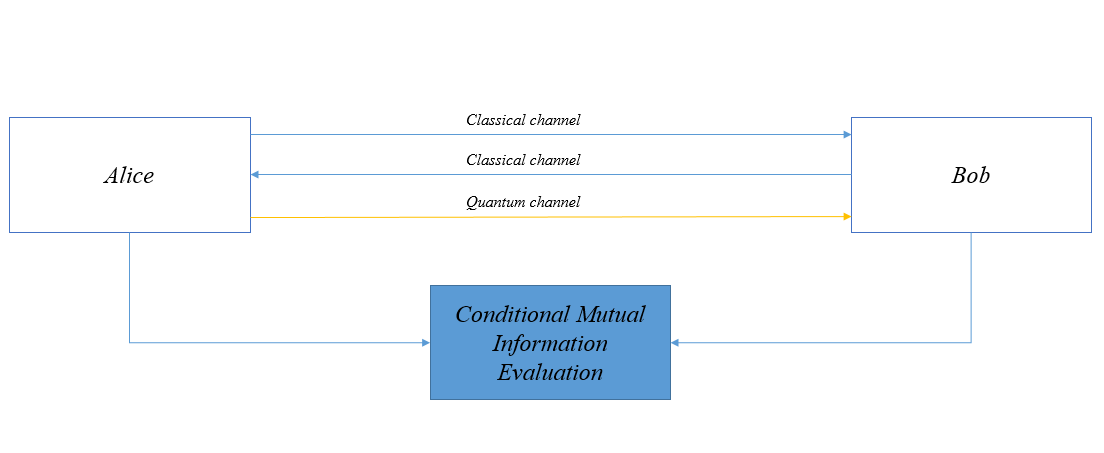
\includegraphics[width=1.0\textwidth, height=11cm]{./sdf/ot_with_discrete_variables/figures/SetupOt.png}
	\caption{Experimental Setup}\label{experimentalsetup}
\end{figure}

As one may see in figure \ref{experimentalsetup} this simulation will have three blocks. Two of them are Alice and Bob and they are connected through two classical channels and one quantum channel. In addition, a third block will be performed for the calculation of \textit{Mutual Information}. The mutual information (MI) between Alice and Bob is defined in terms of their join distribution.

\begin{figure}[h]
	\centering 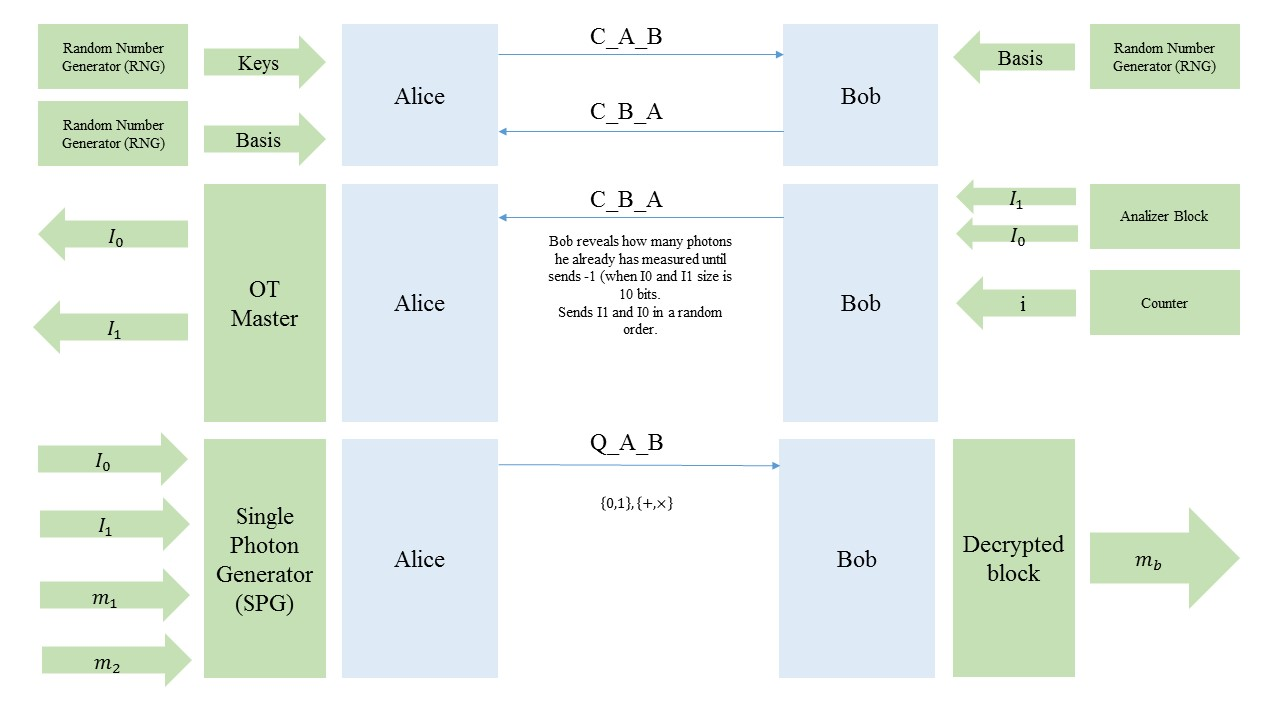
\includegraphics[width=1.1\textwidth,height=9cm]{./sdf/ot_with_discrete_variables/figures/DiagramBlock_Simulation.jpg}
	\caption{Functional Block Diagram}\label{functionalblockdiagram}
\end{figure}

In figure \ref{functionalblockdiagram} is presented the block diagram of the simulation that will be performed. There are two sides (Alice and Bob) and three channels throughout which they will communicate. For classical tasks Alice must have two \textit{Random Number Generators} in order to generate random keys and basis. Likewise, Bob also need to generate the basis through which he will measure the received photons. Next, Bob must have two more blocks, one to analyze and process whether the basis information received by Alice match with his basis information, and another block for photons count. Furthermore, Alice must have a block for \textit{Single Photon Generator} which receives four inputs to encrypt the photons to be sent. Finally, Bob has a block to decrypt messages received by Alice.

\subsection{Experimental}
In figures \ref{quantumchannelcommunication1} and \ref{quantumchannelcommunication2} are presented the experimental setup to be performed in the lab. Starting with Alice's side and then Bob's side.

\begin{figure}[H]
	\centering 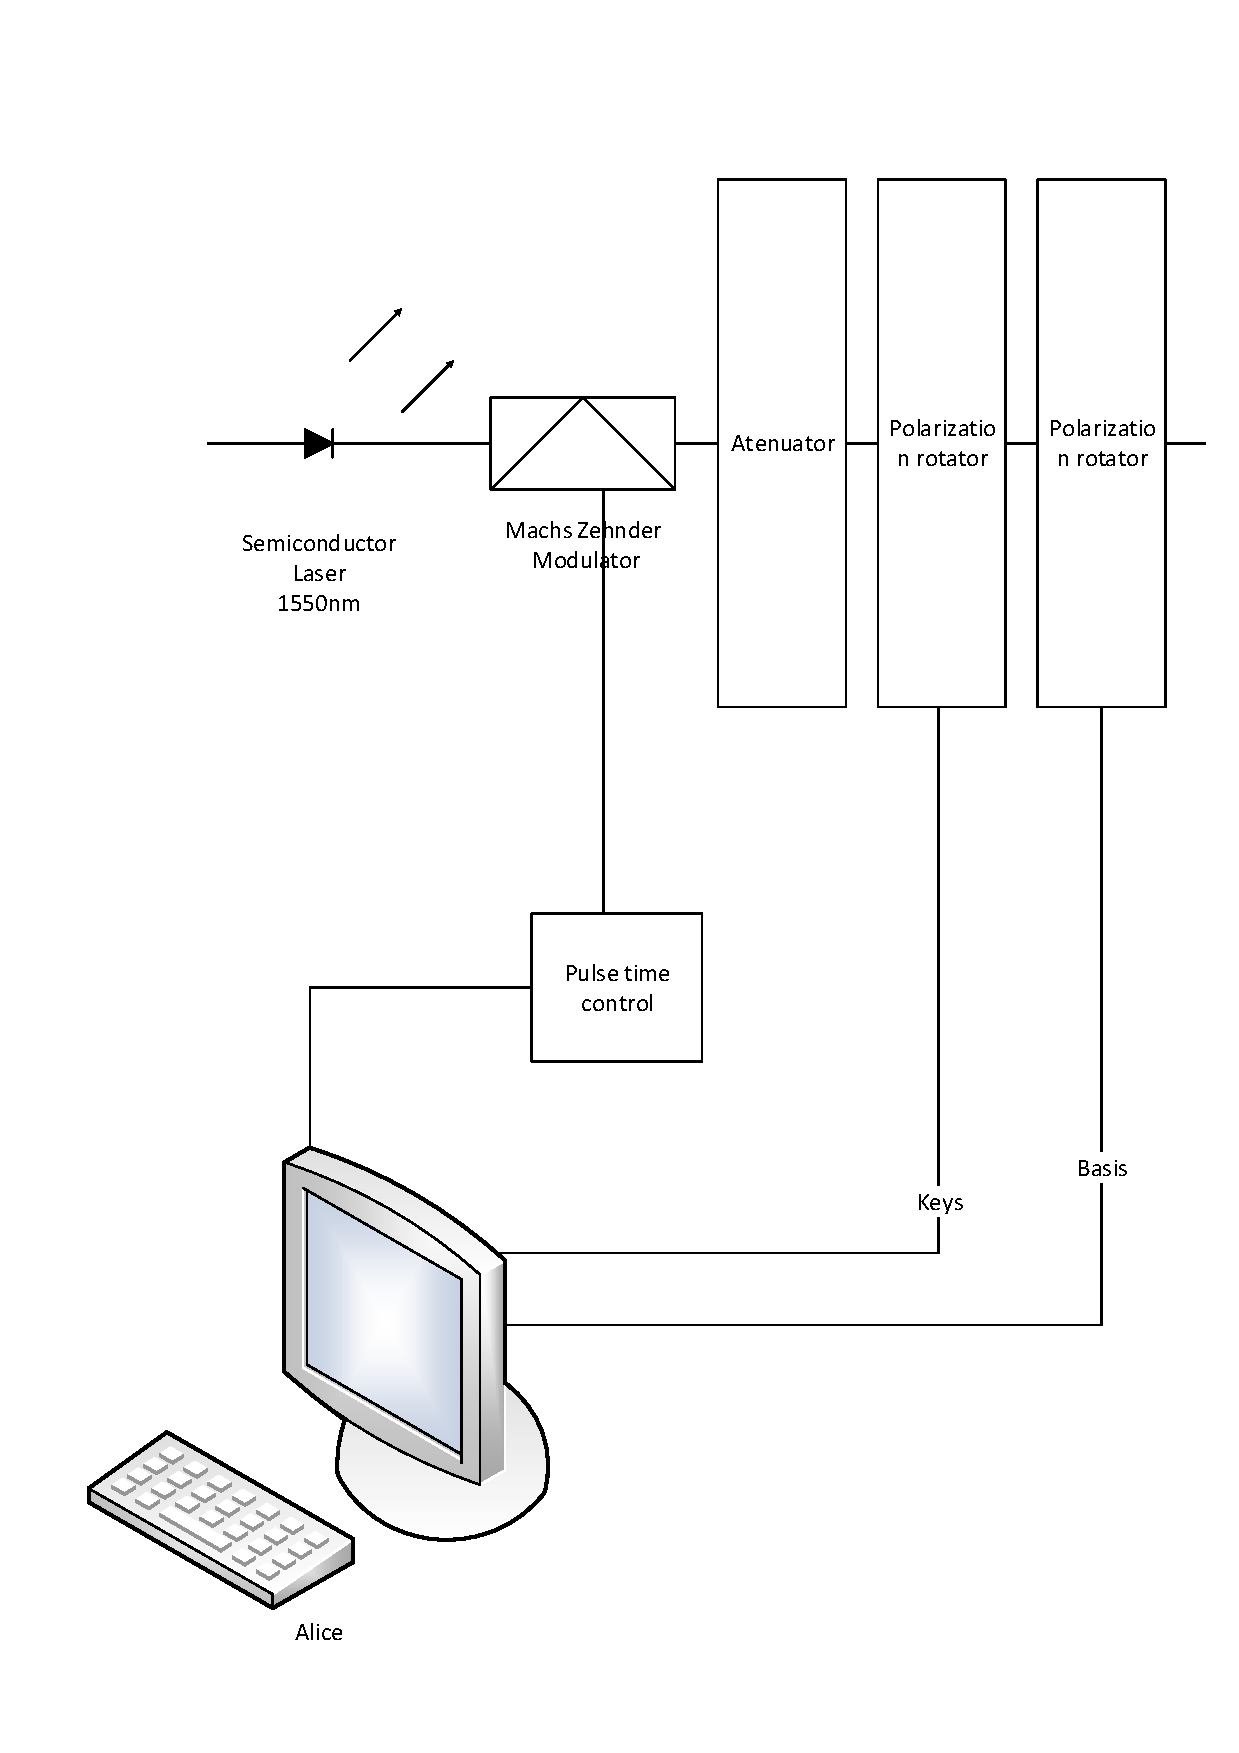
\includegraphics[width=1.1\textwidth,height=20cm]{./sdf/ot_with_discrete_variables/figures/OT_experimental_alice.pdf}
	\caption{Quantum communication diagram - Alice's side}\label{quantumchannelcommunication1}
\end{figure}

\begin{figure}[H]
	\centering 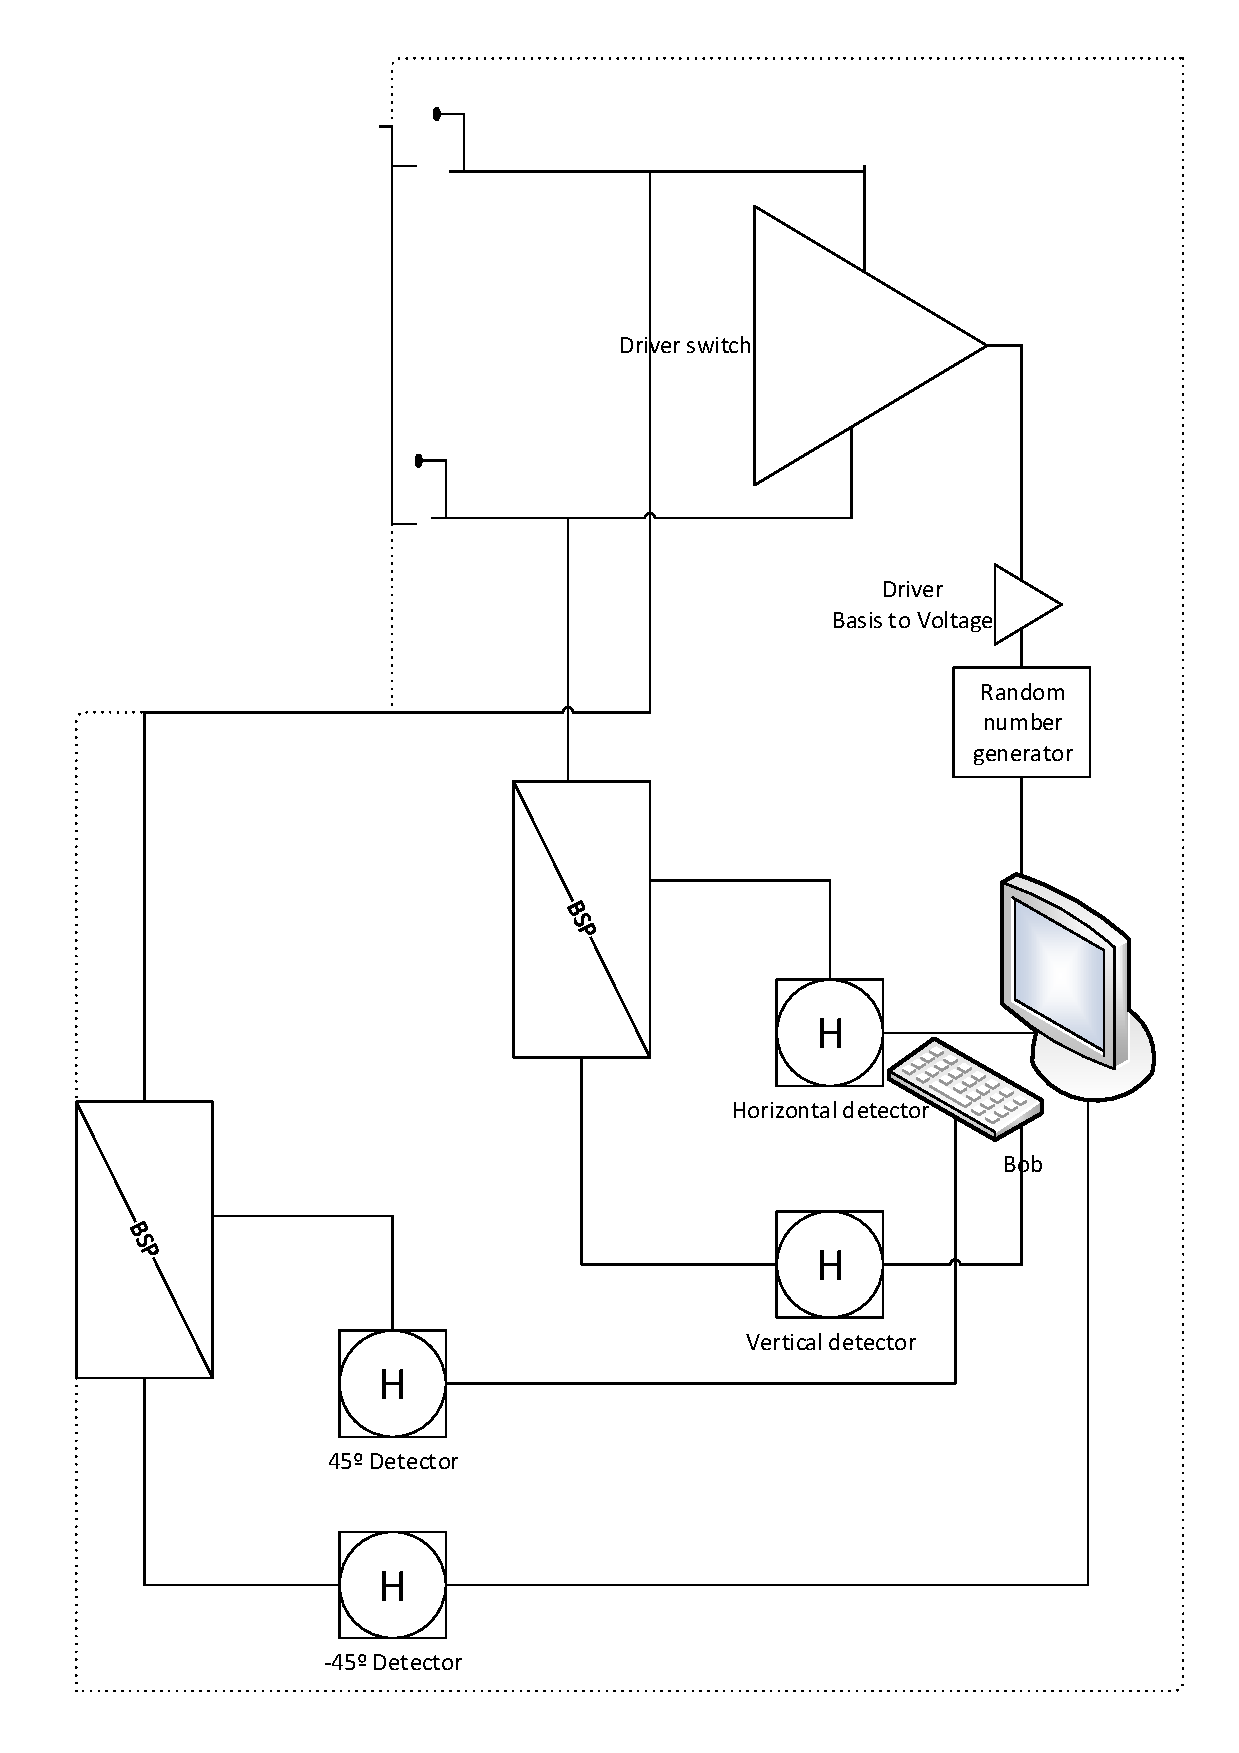
\includegraphics[width=1.1\textwidth,height=20cm]{./sdf/ot_with_discrete_variables/figures/OT_experimental_bob.pdf}
	\caption{Quantum communication diagram - Bob's side}\label{quantumchannelcommunication2}
\end{figure} 
